\documentclass[a4paper]{article}
\usepackage{a4wide,amssymb,epsfig,latexsym,multicol,array,hhline,fancyhdr}
\usepackage{amsmath}
\usepackage{lastpage}
\usepackage[lined,boxed,commentsnumbered]{algorithm2e}
\usepackage{enumerate}
\usepackage{color}
\usepackage{graphicx}							% Standard graphics package
\usepackage{array}
\usepackage{tabularx, caption}
\usepackage{multirow}
\usepackage{multicol}
\usepackage{rotating}
\usepackage{graphics}
\usepackage{geometry}
\usepackage{setspace}
\usepackage{epsfig}
\usepackage{enumitem}
\usepackage{float}
\usepackage{caption}  
\usepackage{indentfirst}

% Required packages and libraries
\usepackage{tikz}
\usetikzlibrary{petri,positioning}
\usetikzlibrary{shapes.geometric}
\usetikzlibrary{automata,positioning,arrows}
\usepackage[utf8]{inputenc}
\usepackage[english]{babel}
\usepackage{hyperref}
\hypersetup{urlcolor=blue,linkcolor=black,citecolor=black,colorlinks=true} 
%\usepackage{pstcol} 								% PSTricks with the standard color package

\newtheorem{theorem}{{\bf Theorem}}
\newtheorem{property}{{\bf Property}}
\newtheorem{proposition}{{\bf Proposition}}
\newtheorem{corollary}[proposition]{{\bf Corollary}}
\newtheorem{lemma}[proposition]{{\bf Lemma}}

\AtBeginDocument{\renewcommand*\contentsname{Contents}}
\AtBeginDocument{\renewcommand*\refname{References}}
%\usepackage{fancyhdr}
\setlength{\headheight}{40pt}
\pagestyle{fancy}
\fancyhead{} % clear all header fields
\fancyhead[L]{
 \begin{tabular}{rl}
    \begin{picture}(25,15)(0,0)
    \put(0,-8){
\includegraphics[width=8mm, height=8mm]{hcmut.png}}
    %\put(0,-8){\epsfig{width=10mm,figure=hcmut.eps}}
   \end{picture}&
	%
\includegraphics[width=8mm, height=8mm]{hcmut.png} & %
	\begin{tabular}{l}
		\textbf{\bf \ttfamily University of Technology, Ho Chi Minh City}\\
		\textbf{\bf \ttfamily Faculty of Computer Science and Engineering}
	\end{tabular} 	
 \end{tabular}
}
\fancyhead[R]{
	\begin{tabular}{l}
		\tiny \bf \\
		\tiny \bf 
	\end{tabular}  }
\fancyfoot{} % clear all footer fields
\fancyfoot[L]{\scriptsize \ttfamily Assignment for Mathematics Modeling - Academic year 2020 - 2021}
\fancyfoot[R]{\scriptsize \ttfamily Page {\thepage}/\pageref{LastPage}}
\renewcommand{\headrulewidth}{0.3pt}
\renewcommand{\footrulewidth}{0.3pt}


%%%
\setcounter{secnumdepth}{4}
\setcounter{tocdepth}{3}
\makeatletter
\newcounter {subsubsubsection}[subsubsection]
\renewcommand\thesubsubsubsection{\thesubsubsection .\@alph\c@subsubsubsection}
\newcommand\subsubsubsection{\@startsection{subsubsubsection}{4}{\z@}%
                                     {-3.25ex\@plus -1ex \@minus -.2ex}%
                                     {1.5ex \@plus .2ex}%
                                     {\normalfont\normalsize\bfseries}}
\newcommand*\l@subsubsubsection{\@dottedtocline{3}{10.0em}{4.1em}}
\newcommand*{\subsubsubsectionmark}[1]{}
%paragraph indentation
\setlength{\parindent}{4em} 

%paragraph spacing
\setlength{\parskip}{0.5em}

%Line spacing
\renewcommand{\baselinestretch}{1.5}
\begin{document}
\begin{titlepage}
	\begin{center}
		VIETNAM NATIONAL UNIVERSITY, HO CHI MINH CITY \\
		UNIVERSITY OF TECHNOLOGY \\
		FACULTY OF COMPUTER SCIENCE AND ENGINEERING
	\end{center}

	\vspace{1cm}

	\begin{figure}[h!]
		\begin{center}
			
\includegraphics[width=3cm]{hcmut.png}
		\end{center}
	\end{figure}

	\vspace{1cm}


	\begin{center}
		\begin{tabular}{c}
			\multicolumn{1}{c}{\textbf{{\Large MATHEMATICAL MODELING (CO2011)}}} \\
			~~                                                                   \\
			\hline
			\\
			\multicolumn{1}{l}{\textbf{{\Large Assignment}}}                     \\
			\\
			\textbf{{\Huge MATHEMATICAL MODELING}}                               \\
			\\
			\textbf{{\Huge and RISK ANALYSIS}}                                   \\
			\\
			\hline
		\end{tabular}
	\end{center}

	\vspace{2cm}

	\begin{table}[h]
		\begin{tabular}{rrl}
			\hspace{5 cm} & Advisor:  & Ph.D Nguyen Tien Thinh         \\
			              & Students: & Le Thong Minh Triet - 2053521. \\
			              &           & Luc Gia Hung - 2053071.        \\
		\end{tabular}
	\end{table}

	\begin{center}
		{\footnotesize HO CHI MINH CITY, NOVEMBER 2021}
	\end{center}
\end{titlepage}


%\thispagestyle{empty}

\newpage
\tableofcontents
\newpage


%%%%%%%%%%%%%%%%%%%%%%%%%%%%%%%%%
\section{Member list \& Workload}

\begin{center}
	\begin{tabular}{|c|c|c|l|c|}
		\hline
		\textbf{No.}       & \textbf{Fullname}                    & \textbf{Student ID}      & \textbf{Problems}                 & \textbf{Percentage of work} \\
		\hline
		%%%%%Student 1%%%%%%%%%%
		\multirow{3}{*}{1} & \multirow{3}{*}{Le Thong Minh Triet} & \multirow{3}{*}{2053521} & - Text                            & \multirow{3}{*}{40\%}       \\
		                   &                                      &                          & Text.                             &                             \\
		                   &                                      &                          & - Text.                           &                             \\
		\hline
		%%%%%Student 2%%%%%%%%%%%
		\multirow{3}{*}{2} & \multirow{3}{*}{Luc Gia Hung}        & \multirow{3}{*}{2053071} & - Relation \& Counting: 4, 5, 6   & \multirow{3}{*}{20\%}       \\
		                   &                                      &                          & Bonus: 4, 5, 6.                   &                             \\
		                   &                                      &                          & - Graph: 1, 2, 3, Bonus: 1, 2, 3. &                             \\
		\hline
	\end{tabular}
\end{center}
\newpage
%%%%%%%%%%%%%%%%%%%%%%%%%%%%%%%%%
\section{Background}
\indent Petri nets have been in the best position to shape some foreseeable developing lines of computer science and
to contribute to novel concepts like “model-based,” “ubiquitous,”
“pervasive” or “disappearing” software engineering. Petri nets and their extensions are promising methods for modeling and simulating
huge systems such as Clinic or Hospital systems. In this assignment, we will study the Petri nets and their applications in the context of computer science.
%%%%%%%%%%%%%%%%%%%%%%%%%%%%%%%%%
\section{Introduction To Assignment}
\par
SCENARIO: Under a SARS pandemic where a huge lack of ICU beds occurs in city H,
patients should consult specialists in the outpatient clinic of a hospital, we describe the
course of business around a specialist in this outpatient clinic of hospital X as a process
model, formally, we use Petri Net.\par
%%%%%%%%%%%%%%%%%%%%%%%%%%%%%%%%%
\section{Solving Assignment Problem}
\subsection{Problem 1}
\begin{figure}[H]
	\centering
	\begin{tikzpicture}[node distance=3cm,on grid]

		% Place 1
		\node[place,
			fill=orange!25,
			draw=orange!75,
			tokens=1,
			label=above:$Free$] (place1) {};
		% Transition 1
		\node[transition,
			below = 1.5cm and 2cm of place1,
			minimum size=0.75cm,
			label=below:$Start$] (trans1) {};
		% Place 2
		\node[place,
			fill=orange!25,
			draw=orange!75,
			right = 2cm of trans1,
			label=below:$Busy$] (place2) {};
		% Transition 2
		\node[transition,
			right = 2cm of place1,
			minimum size=0.75cm,
			label=above:$End$] (trans2) {};
		% Place 2
		\node[place,
			fill=orange!25,
			draw=orange!75,
			right = 2cm of trans2,
			label=above:$Docu$] (place3) {};
		% Transition 3
		\node[transition,
			right = 2cm of place2,
			minimum size=0.75cm,
			label=below:$Change$] (trans3) {};
		% Connect P-T-P
		\draw[thick] (place1) edge[post] (trans1) (trans1) edge[post] (place2)
		(place2) edge[post] (trans3) (trans3) edge[post] (place3)
		(place3) edge[post] (trans2) (trans2) edge[post] (place1);
	\end{tikzpicture}
\end{figure}

\begin{enumerate}[label=(\alph*)]

	\item State: Free, Busy, Docu\\
	      Transition: Start, End, Change
	\item \begin{enumerate}[label=(\roman*)]
		      \item Figure of transition system that each place cannot contain more than one token in any marking are represented below.\\
		            \begin{figure}[H]
			            \centering
			            \begin{tikzpicture}
				            \node[ellipse, draw] (vertex1){1, 0, 0};
				            \node[ellipse, draw, below left = 1.5cm and 2 cm of vertex1] (vertex2){0, 1, 0};
				            \node[ellipse, draw, below right = 1.5cm and 2 cm of vertex1] (vertex3){0, 0, 1};
				            \draw[->]
				            (vertex1)    edge[post,bend right=20]  node[sloped, anchor=center, above, text width=1.0cm] {Start}     (vertex2)
				            (vertex2)    edge[post,bend right=20]  node[sloped, anchor=center, above, text width=1.0cm] {Change}     (vertex3)
				            (vertex3)    edge[post,bend right=20]  node[sloped, anchor=center, above, text width=1.0cm] {End}     (vertex1);
			            \end{tikzpicture}
			            \caption{State of the system}
			            \label{fig:M1}
		            \end{figure}
		            \begin{figure}[H]
			            \centering
			            \begin{tikzpicture}
				            \node[ellipse, draw] (vertex1){1, 1, 0};
				            \node[ellipse, draw, below left = 1.5cm and 2 cm of vertex1] (vertex2){0, 2, 0};
				            \node[ellipse, draw, below right = 1.5cm and 2 cm of vertex1] (vertex3){1, 0, 1};
				            \node[ellipse, draw, below = 1.5cm of vertex3] (vertex4){2, 0, 0};
				            \node[ellipse, draw, below = 1.5cm of vertex2] (vertex5){0, 1, 1};
				            \node[ellipse, draw, below left = 1.5cm and 2 cm of vertex4] (vertex6){0, 0, 2};

				            \draw[->]
				            (vertex1)    edge[post,bend right=20]  node[sloped, anchor=center, above, text width=1.0cm] {Start}     (vertex2)
				            (vertex1)    edge[post,bend left=20]  node[sloped, anchor=center, above, text width=1.0cm] {Change}     (vertex3)
				            (vertex2)    edge[post]  node[sloped, anchor=center, above, text width=1.0cm] {Change}     (vertex5)
				            (vertex3)    edge[post]  node[sloped, anchor=center, above, text width=1.0cm] {End}     (vertex4)
				            (vertex3)    edge[post]  node[sloped, anchor=center, above, text width=1.0cm] {Start}     (vertex5)
				            (vertex5)    edge[post,bend right=20]  node[sloped, anchor=center, above, text width=1.0cm] {Change}     (vertex6)
				            (vertex5)    edge[post,bend right=20]  node[sloped, anchor=center, above, text width=1.0cm] {End}     (vertex1)
				            (vertex6)    edge[post]  node[sloped, anchor=center, above, text width=1.0cm] {End}     (vertex3)
				            (vertex4)    edge[post] node[sloped, anchor=center, above, text width=1.0cm] {Start}     (vertex1);
			            \end{tikzpicture}
			            \caption{State of the system}
			            \label{fig:M2}
		            \end{figure}
		            \begin{figure}[H]
			            \centering
			            \begin{tikzpicture}
				            \node[ellipse, draw] (vertex1){1, 1, 1};
				            \node[ellipse, draw, right = 2cm of vertex1] (vertex2){2, 1, 0};
				            \node[ellipse, draw, below right = 2cm of vertex2] (vertex3){2, 0, 1};
				            \node[ellipse, draw, below right = 2cm of vertex3] (vertex4){3, 0, 0};
				            \node[ellipse, draw, below left = 2cm of vertex4] (vertex5){0, 3, 0};
				            \node[ellipse, draw, below left = 2cm of vertex5] (vertex6){0, 0, 3};
				            \node[ellipse, draw, below left = 2cm of vertex1] (vertex7){0, 2, 1};
				            \node[ellipse, draw, below left = 2cm of vertex7] (vertex8){1, 0, 2};
				            \node[ellipse, draw, below right = 2cm of vertex8] (vertex9){0, 1, 2};
				            \node[ellipse, draw, below right = 2cm of vertex9] (vertex10){1, 2, 0};
				            \draw[->]
				            (vertex1)    edge[post]  node[sloped, anchor=center, above, text width=1.0cm] {End}     (vertex2)
				            (vertex1)    edge[post]  node[sloped, anchor=center, above, text width=1.0cm] {Start}     (vertex7)
				            (vertex1)    edge[post, bend right=30]  node[sloped, anchor=center, above, text width=1.0cm] {Change}     (vertex8)
				            (vertex2)    edge[post]  node[sloped, anchor=center, above, text width=1.0cm] {Start}     (vertex10)
				            (vertex2)    edge[post]  node[sloped, anchor=center, above, text width=1.0cm] {Change}     (vertex3)
				            (vertex3)    edge[post,bend left=20]  node[sloped, anchor=center, above, text width=1.5cm] {Start}     (vertex1)
				            (vertex3)    edge[post]  node[sloped, anchor=center, above, text width=1.5cm] {End}     (vertex4)
				            (vertex4)    edge[post,bend left = 30]  node[sloped, anchor=center, above, text width=1.5cm] {Start}     (vertex1)
				            (vertex5)    edge[post,bend left = 30]  node[sloped, anchor=center, above, text width=2.5cm] {Change}     (vertex7)
				            (vertex6)    edge[post,bend right = 10]  node[sloped, anchor=center, above, text width=1.5cm] {End}     (vertex8)
				            (vertex8)    edge[post]  node[sloped, anchor=center, below, text width=1.0cm] {Start}     (vertex9)
				            (vertex8)    edge[post]  node[sloped, anchor=center, above, text width=1.0cm] {End}     (vertex3)
				            (vertex7)    edge[post]  node[sloped, anchor=center, above, text width=1.0cm] {Change}     (vertex9)
				            (vertex7)    edge[post]  node[sloped, anchor=center, above, text width=1.5cm] {End}     (vertex10)
				            (vertex9)    edge[post,bend right=50]  node[sloped, anchor=center, below, text width=2.5cm] {Change}     (vertex6)
				            (vertex9)    edge[post]  node[sloped, anchor=center, above, text width=0cm] {End}     (vertex1)
				            (vertex10)    edge[post]  node[sloped, anchor=center, above, text width=0cm] {Start}     (vertex5)
				            (vertex10)    edge[post]  node[sloped, anchor=center, above, text width=0.8cm] {Change}     (vertex1);
			            \end{tikzpicture}
			            \caption{State of the system}
			            \label{fig:M3}
		            \end{figure}
		      \item According to  Fig.~\ref{fig:M1},  Fig.~\ref{fig:M2} and  Fig.~\ref{fig:M3}, every triplet (x, y, z) creates a transition system that every vertex is a triplet of nonnegative integers $(x_0, y_0, z_0)$ such that:\\
		            \[x_0 + y_0 + z_0 = x + y + z\]\\
		            So, we can represent the transition system with the given triplet (x, y, z) by finding number of ways to write $S = x + y + z $ as a sum of three integers.\par
		            This can be solve by thinking recursively and using induction.\par
		            Let $F_k(n)$ be the number of ways to sum $k$ natural numbers so the sum is $n$.

		            Assume we have three numbers we want to sum to 4. The number of ways to do this is the same as setting the first digit to
		            \textbf{k= 4, 3, 2, 1, 0}  in turn and then using remaining digits to sum up \textbf{k - 1}\\
		            Number of ways to write 4 with three digits =\par

		            {4 + {number of ways to write 0 with two digits}} +\par

		            {3 + {number of ways to write 1 with two digits}} +\par

		            {2 + {number of ways to write 2 with two digits}} +\par

		            {1 + {number of ways to write 3 with two digits}} +\par

		            {0 + {number of ways to write 4 with two digits}}\par
		            Which is the same as writing (in our notation):
		            \[F_3(4)=F_2(0)+F_2(1)+F_2(2)+F_2(3)+F_2(4)\]
		            For the general case we have:
		            \[F_k(n) = \sum_{l = 0}^{n}F_{k-1}(l)  \]
		            It is also easily seen that $F_1(n) = 1$ and $F_k(0) = 1$. This now allows us to expand the first few relations as
		            \begin{align*}
			            F_1(n) & =  1                                                         \\
			            F_2(n) & =  \sum_{l = 0}^{n}F_1(l) = \frac{n + 1}{1!}                 \\
			            F_3(n) & =  \sum_{l = 0}^{n}F_2(l) = \frac{{(n + 1)}^2 + (n + 1)}{2!}
		            \end{align*}
	      \end{enumerate}
\end{enumerate}


\subsection{Problem 2}
\begin{enumerate}[label=(\alph*)]
	\item Number of tokens in state $N_{Pa}$ shows quantity of patients are treating by the specialist.
	\item Petri net $N_{Pa}$ which contains five patients in state wait, no
	patient in state inside, and one patient is in state done are represented by the following graph:
\end{enumerate}
\begin{figure}[H]
	\centering
	
\begin{tikzpicture}
		% Petri Net illustration Code
		% Place 1
		\node[place,
			fill=orange!25,
			draw=orange!75,
			tokens=5,
			label=below:$Wait$] (place1) at (0,0) {};

		% Place 2
		\node[place,
			fill=orange!25,
			draw=orange!75,
			label=below:$Inside$] (place2)  at (4,0) {};
		% Place 3
		\node[place,
			fill=orange!25,
			draw=orange!75,
			tokens=1,
			label=below:$Done$] (place3)  at (8,0) {};
		% Transition 1
		\node[transition,
			minimum size=0.75cm,
			label=above:$Start$] (Trans1) at (2,0) {};
		% Transition2
		\node[transition,
			minimum size=0.75cm,
			label=above:$Change$] (Trans2) at (6,0) {};
		% Connect P-T-P
		\draw[thick]
		(Trans1) edge[post] (place2) (Trans2) edge[post] (place3)
		(place1) edge[post] (Trans1) (place2) edge[post] (Trans2);

	\end{tikzpicture}
	\caption{Petri Net for patients}
\end{figure}
\begin{figure}[H]
	\centering
	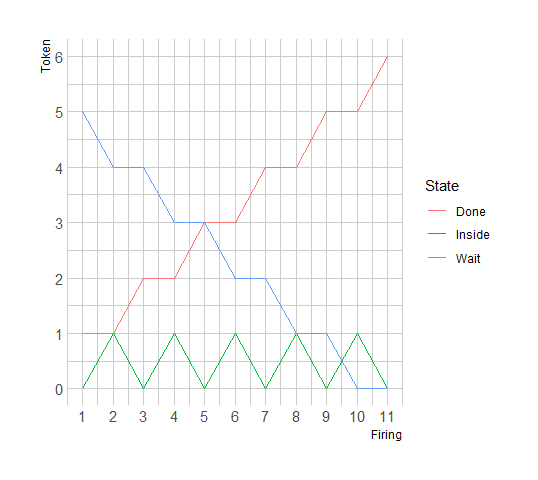
\includegraphics[width=\linewidth]{QUES2.png}
	\caption{Marking of the Petri Net when firing}
	\label{fig:q2}
\end{figure}
\subsection{Problem 3}
\begin{figure}[H]
	\centering
	\begin{tikzpicture}[node distance=3cm,on grid]

		% Place 1
		\node[place,
			fill=orange!25,
			draw=orange!75,
			tokens=1,
			label=below:$Free$] (place1) {};

		% Place 2
		\node[place,
			below=of place1,
			fill=orange!25,
			draw=orange!75,
			tokens=4,
			label=below:$Wait$] (place2) {};
		% Transition 1
		\node[transition,
			below right= 1.5cm and 2cm of place1,
			minimum size=0.75cm,
			label=above:$Start$] (trans1) {};
		% Place 3
		\node[place,
			above right= 1.5cm and 2cm of trans1,
			fill=orange!25,
			draw=orange!75,
			tokens=0,
			label=below:$Busy$] (place3) {};
		% Place 4
		\node[place,
			below right= 1.5cm and 2cm of trans1,
			fill=orange!25,
			draw=orange!75,
			tokens=0,
			label=below:$Inside$] (place4) {};
		% Transition 2
		\node[transition,
			below right= 1.5cm and 2cm of place3,
			minimum size=0.75cm,
			label=above:$Change$] (trans2) {};
		% Place 5
		\node[place,
			above right= 1.5cm and 2cm of trans2,
			fill=orange!25,
			draw=orange!75,
			tokens=0,
			label=below:$Docu$] (place5) {};
		% Place 6
		\node[place,
			below right= 1.5cm and 2cm of trans2,
			fill=orange!25,
			draw=orange!75,
			tokens=1,
			label=below:$Done$] (place6) {};
		% Transition 3
		\node[transition,
			above = 1.5cm of place3,
			minimum size=0.75cm,
			label=above:$End$] (trans3) {};
		% Connect P-T-P
		\draw[thick] (place1) edge[post] (trans1) (place2) edge[post] (trans1)
		(place3) edge[post] (trans2) (place4) edge[post] (trans2)
		(trans1) edge[post] (place3) (trans1) edge[post] (place4)
		(trans2) edge[post] (place5) (trans2) edge[post] (place6)
		(place5) edge[post,bend right=20] (trans3) (trans3) edge[post,bend right=20] (place1);
	\end{tikzpicture}
	\caption{Petri Net for the problem 3}
\end{figure}
\begin{figure}[H]
	\centering
	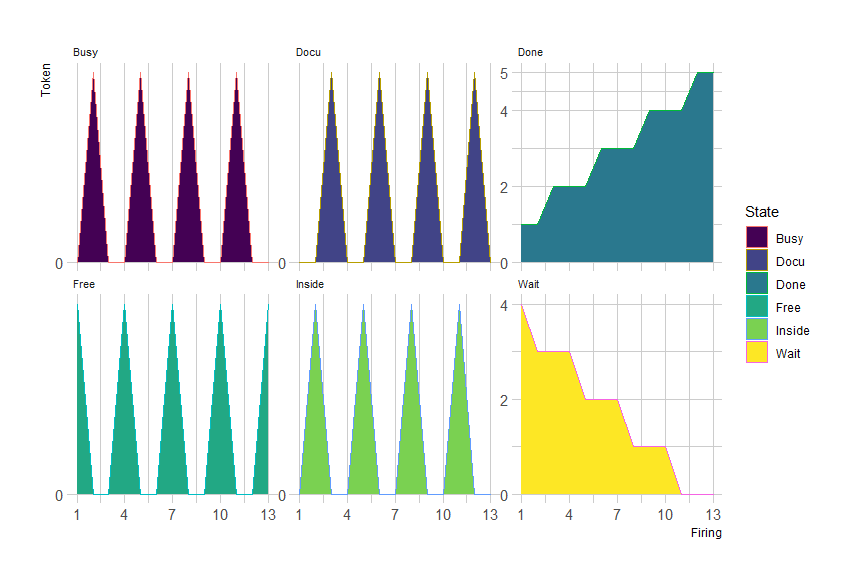
\includegraphics[width=\linewidth]{QUES3.png}
	\caption{Marking of the Petri Net when firing}
	\label{fig:q3}
\end{figure}
\subsection{Problem 4}
\begin{figure}[H]
	\centering
	\begin{tikzpicture}[node distance=3cm,on grid]

		% Place 1
		\node[place,
			fill=orange!25,
			draw=orange!75,
			tokens=1,
			label=below:$Free$] (place1) {};

		% Place 2
		\node[place,
			below=of place1,
			fill=orange!25,
			draw=orange!75,
			tokens=3,
			label=below:$Wait$] (place2) {};
		% Transition 1
		\node[transition,
			below right= 1.5cm and 2cm of place1,
			minimum size=0.75cm,
			label=above:$Start$] (trans1) {};
		% Place 3
		\node[place,
			above right= 1.5cm and 2cm of trans1,
			fill=orange!25,
			draw=orange!75,
			tokens=0,
			label=below:$Busy$] (place3) {};
		% Place 4
		\node[place,
			below right= 1.5cm and 2cm of trans1,
			fill=orange!25,
			draw=orange!75,
			tokens=0,
			label=below:$Inside$] (place4) {};
		% Transition 2
		\node[transition,
			below right= 1.5cm and 2cm of place3,
			minimum size=0.75cm,
			label=above:$Change$] (trans2) {};
		% Place 5
		\node[place,
			above right= 1.5cm and 2cm of trans2,
			fill=orange!25,
			draw=orange!75,
			tokens=0,
			label=below:$Docu$] (place5) {};
		% Place 6
		\node[place,
			below right= 1.5cm and 2cm of trans2,
			fill=orange!25,
			draw=orange!75,
			tokens=1,
			label=below:$Done$] (place6) {};
		% Transition 3
		\node[transition,
			above = 1.5cm of place3,
			minimum size=0.75cm,
			label=above:$End$] (trans3) {};
		% Connect P-T-P
		\draw[thick] (place1) edge[post] (trans1) (place2) edge[post] (trans1)
		(place3) edge[post] (trans2) (place4) edge[post] (trans2)
		(trans1) edge[post] (place3) (trans1) edge[post] (place4)
		(trans2) edge[post] (place5) (trans2) edge[post] (place6)
		(place5) edge[post,bend right=20] (trans3) (trans3) edge[post,bend right=20] (place1);
	\end{tikzpicture}
	\caption{The Petri net for the problem 4.}
\end{figure}
\begin{figure}[H]
	\centering
	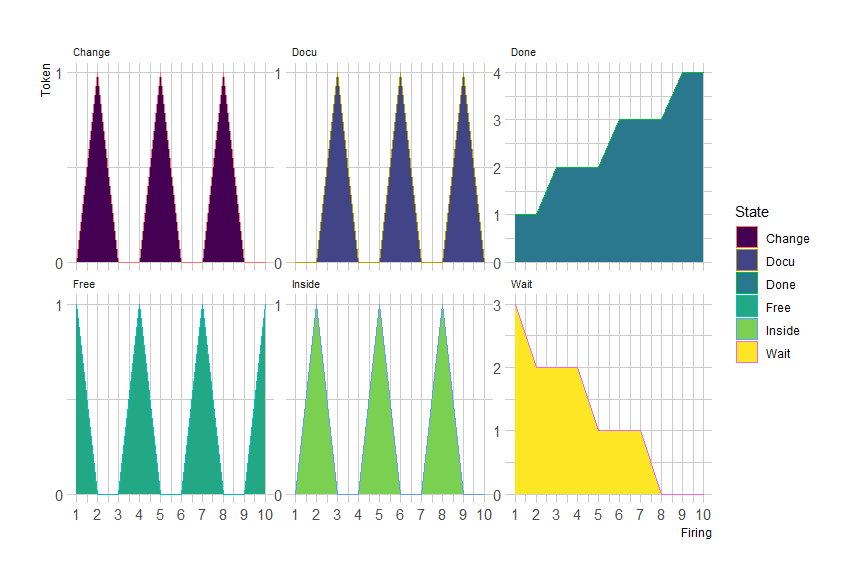
\includegraphics[width=12cm]{QUES4.png}
	\caption{Marking of the Petri net when firing once}
	\label{fig:q4}
\end{figure}
From the Fig.~\ref{fig:q4}, we can see all places are reachable because there is always a sequence of steps to each place.
\subsection{Problem 5}
The superimposed Petri net N is not deadlock free because state Done is not the state of at least one node. Therefore, there is not a node is enabled in state Done
\subsection{Problem 6}
\begin{figure}[H]
	\centering
	\begin{tikzpicture}[node distance=3cm,on grid]
		% Place 1
		\node[ellipse, draw,minimum size=1cm,label={-135:$INT$}] (place1){Free};
		\node[rectangle, draw, above left = 0.69cm and 0.67cm of place1,minimum width = 0.2cm,
			minimum height = 0.1cm] (p1) {1' 2};
		%%%%%% VARIABLE %%%%%%
		\node[rectangle,above left = 4 cm of place1,minimum width = 2cm,
			minimum height = 1cm,text width=9.0cm] (p3) {COL: INT = int\\
			COL: SPEC = union $S_1$: INT + $S_2$: INT\\
			var i: INT\\
			var s: SPEC};
		% Transition 1
		\node[transition,
			right= 4cm of place1,
			minimum size=0.75cm,text width=1cm,align=center
		] (trans1) {$S_1$};
		% Transition 2
		\node[transition,
			above= 2cm of trans1,
			minimum size=0.75cm,text width=1cm,align=center
		] (trans2) {$S_2$};
		% Place 2
		\node[ellipse, right = 4cm of trans1 ,draw,minimum size=1cm,label={-45:$SPEC$}] (place2){Busy};
		% Transition
		\node[transition,
			below= 3cm of place2,
			minimum size=0.75cm,text width=1.5cm,align=center
		] (trans3) {Change};
		% Place 3
		\node[ellipse, below = 3cm of trans3 ,draw,minimum size=1cm,label={-45:$SPEC$}] (place3){Docu};
		% Transition 4
		\node[transition,
			left= 4cm of trans3,
			minimum size=0.75cm,text width=1.5cm,align=center
		] (trans4) {End};
		\draw[->]
		(place1)    edge[post]  node[sloped, anchor=center, above, text width=1.0cm] {i - 1}     (trans1)
		(place1)    edge[post,bend left=30]  node[sloped, anchor=center, above, text width=1.0cm] {i - 1}     (trans2)
		(trans2)    edge[post,bend left=28]  node[sloped, anchor=center, above, text width=1.0cm] {$S_2(i)$}     (place2)
		(trans1)    edge[post]  node[sloped, anchor=center, above, text width=1.0cm] {$S_1(i)$}     (place2)
		(place2)    edge[post]  node[align=center, anchor=center, left, text width=0.3cm] {s}     (trans3)
		(trans3)    edge[post]  node[align=center, anchor=center, left, text width=0.3cm] {s}     (place3)
		(place3)    edge[post]  node[align=center, anchor=center, left, text width=0.3cm] {s}     (trans4)
		(trans4)    edge[post]  node[sloped, anchor=center, below, text width=1.0cm] {i + 1}     (place1)
		;
	\end{tikzpicture}
	\caption{CPN for two specialists}
	\label{fig:cpn}
\end{figure}
ASSUMPTION:\par
Two specialists are distinguished and working in the same process.\par
There are three places in Fig.~\ref{fig:cpn}: Free, Busy and Docu. A transition represents an action of this business process. Graphically, a rectangle
represents a transition. The CPN in Fig..~\ref{fig:cpn} has four transitions: S1, S2, Change and End.\par
In Fig.~\ref{fig:cpn}, place FREE is of type INT and two remaining places are of type SPEC (union of two type S1 and S2). Type S1 and S2 indicate that the Specialist
is $Specialist_1(S_1)$ or the $Specialist_2(S_2)$


%%%%%%%%%%%%%%%%%%%%%%%%%%%%%%%%%
\newpage
\begin{thebibliography}{80}


	\bibitem{bib1}
	...


	\bibitem{bib2}
	...


\end{thebibliography}
\end{document}

